\documentclass{beamer}
\usepackage{graphicx}
\usepackage{subfig}
\usepackage{amsmath}
\usepackage{amssymb}
\usepackage{pifont}
\newcommand{\cmark}{\ding{51}}%
\newcommand{\xmark}{\ding{55}}%
\newcommand{\done}{\item[\cmark]}
\newcommand{\crossed}{\item[\xmark]}
\usepackage{xcolor}
\usepackage{hyperref}

\hypersetup{
    colorlinks=true,
    urlcolor=blue
}


\title{Future of Voice Agents}
\author{Christopher Hong}

\begin{document}

\frame{\titlepage}

\begin{frame}
\frametitle{Observation, Values and Mission}
\begin{itemize}
    \item The advent of large language models have enabled a new bridge between everyday people and computing
    \item AI should allow everyday people to harness the power of computation
    \item People should be in control of their computing, not vice versa
\end{itemize}
\end{frame}

\begin{frame}
\frametitle{Big Tech Voice Assistants (Alexa, Gemini, Siri)...}
\begin{itemize}
    \done Do well at some basic pre-programmed tasks
    \crossed Don't grasp the context of voice commands
    \crossed Don't integrate well or at all with third-party applications
    \crossed Fail to transcribe words accurately that humans have no problem given a situational context (ex. "hot words" in speech recognition research)
    \crossed Don't compose appropriate action for more complex user requests
\end{itemize}
\end{frame}

\begin{frame}
\frametitle{Solution}
\begin{itemize}
    \item Bridge user-intent to application-specific code using (large) language models
    \item Imbue automatic speech recognition with contextual capability for short-form transcription
    \item Give application developers the tools to contextualize voice assistance
\end{itemize}
\end{frame}

\begin{frame}
\frametitle{Prototype case: Gym Working Logging App}
\begin{columns}
\begin{column}{0.5\textwidth}
    Suppose, in a workout logging app, the user wants to switch to recording a different type (eg. "Ab Crunch Machine"). How can the user invoke a voice assistant to specify it quickly?
    \vspace{2cm}
\end{column}
\begin{column}{0.5\textwidth}
    \centering
    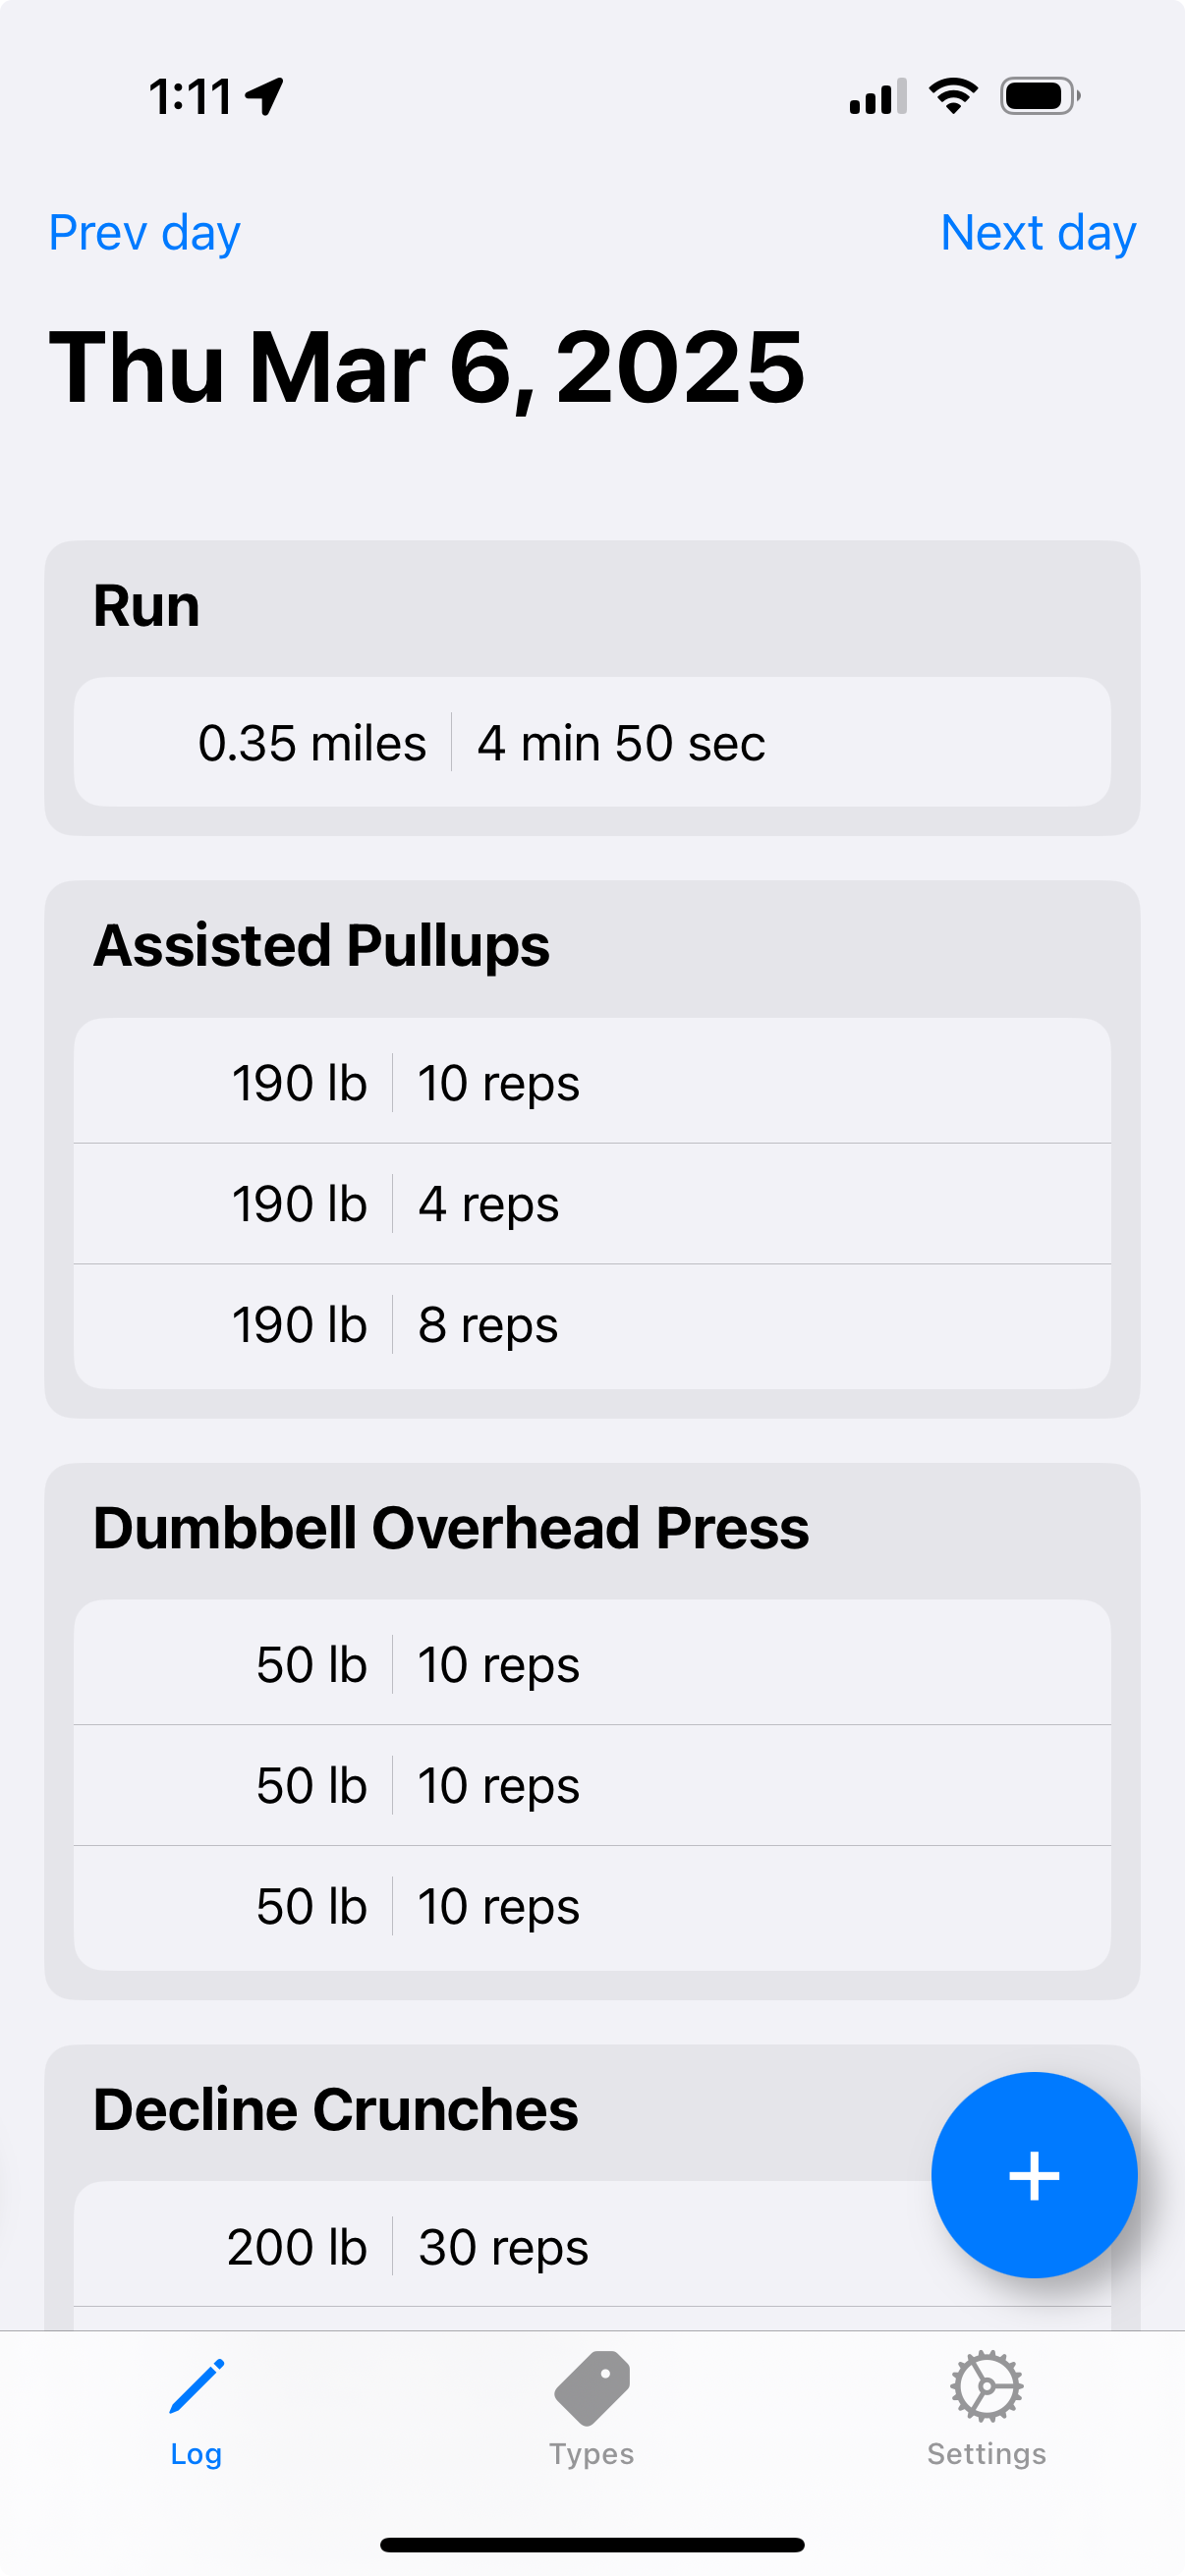
\includegraphics[height=8cm]{images/sc.png}
\end{column}
\end{columns}
\end{frame}

\begin{frame}
\frametitle{Prototype case: Gym Working Logging App}
\begin{columns}
\begin{column}{0.5\textwidth}
    Instead of using a platform or SaaS API from Apple, Google, etc., use a tailored automatic speech recognition pipeline to control quality and viability.
    \vspace{2cm}
\end{column}
\begin{column}{0.5\textwidth}
    \centering
    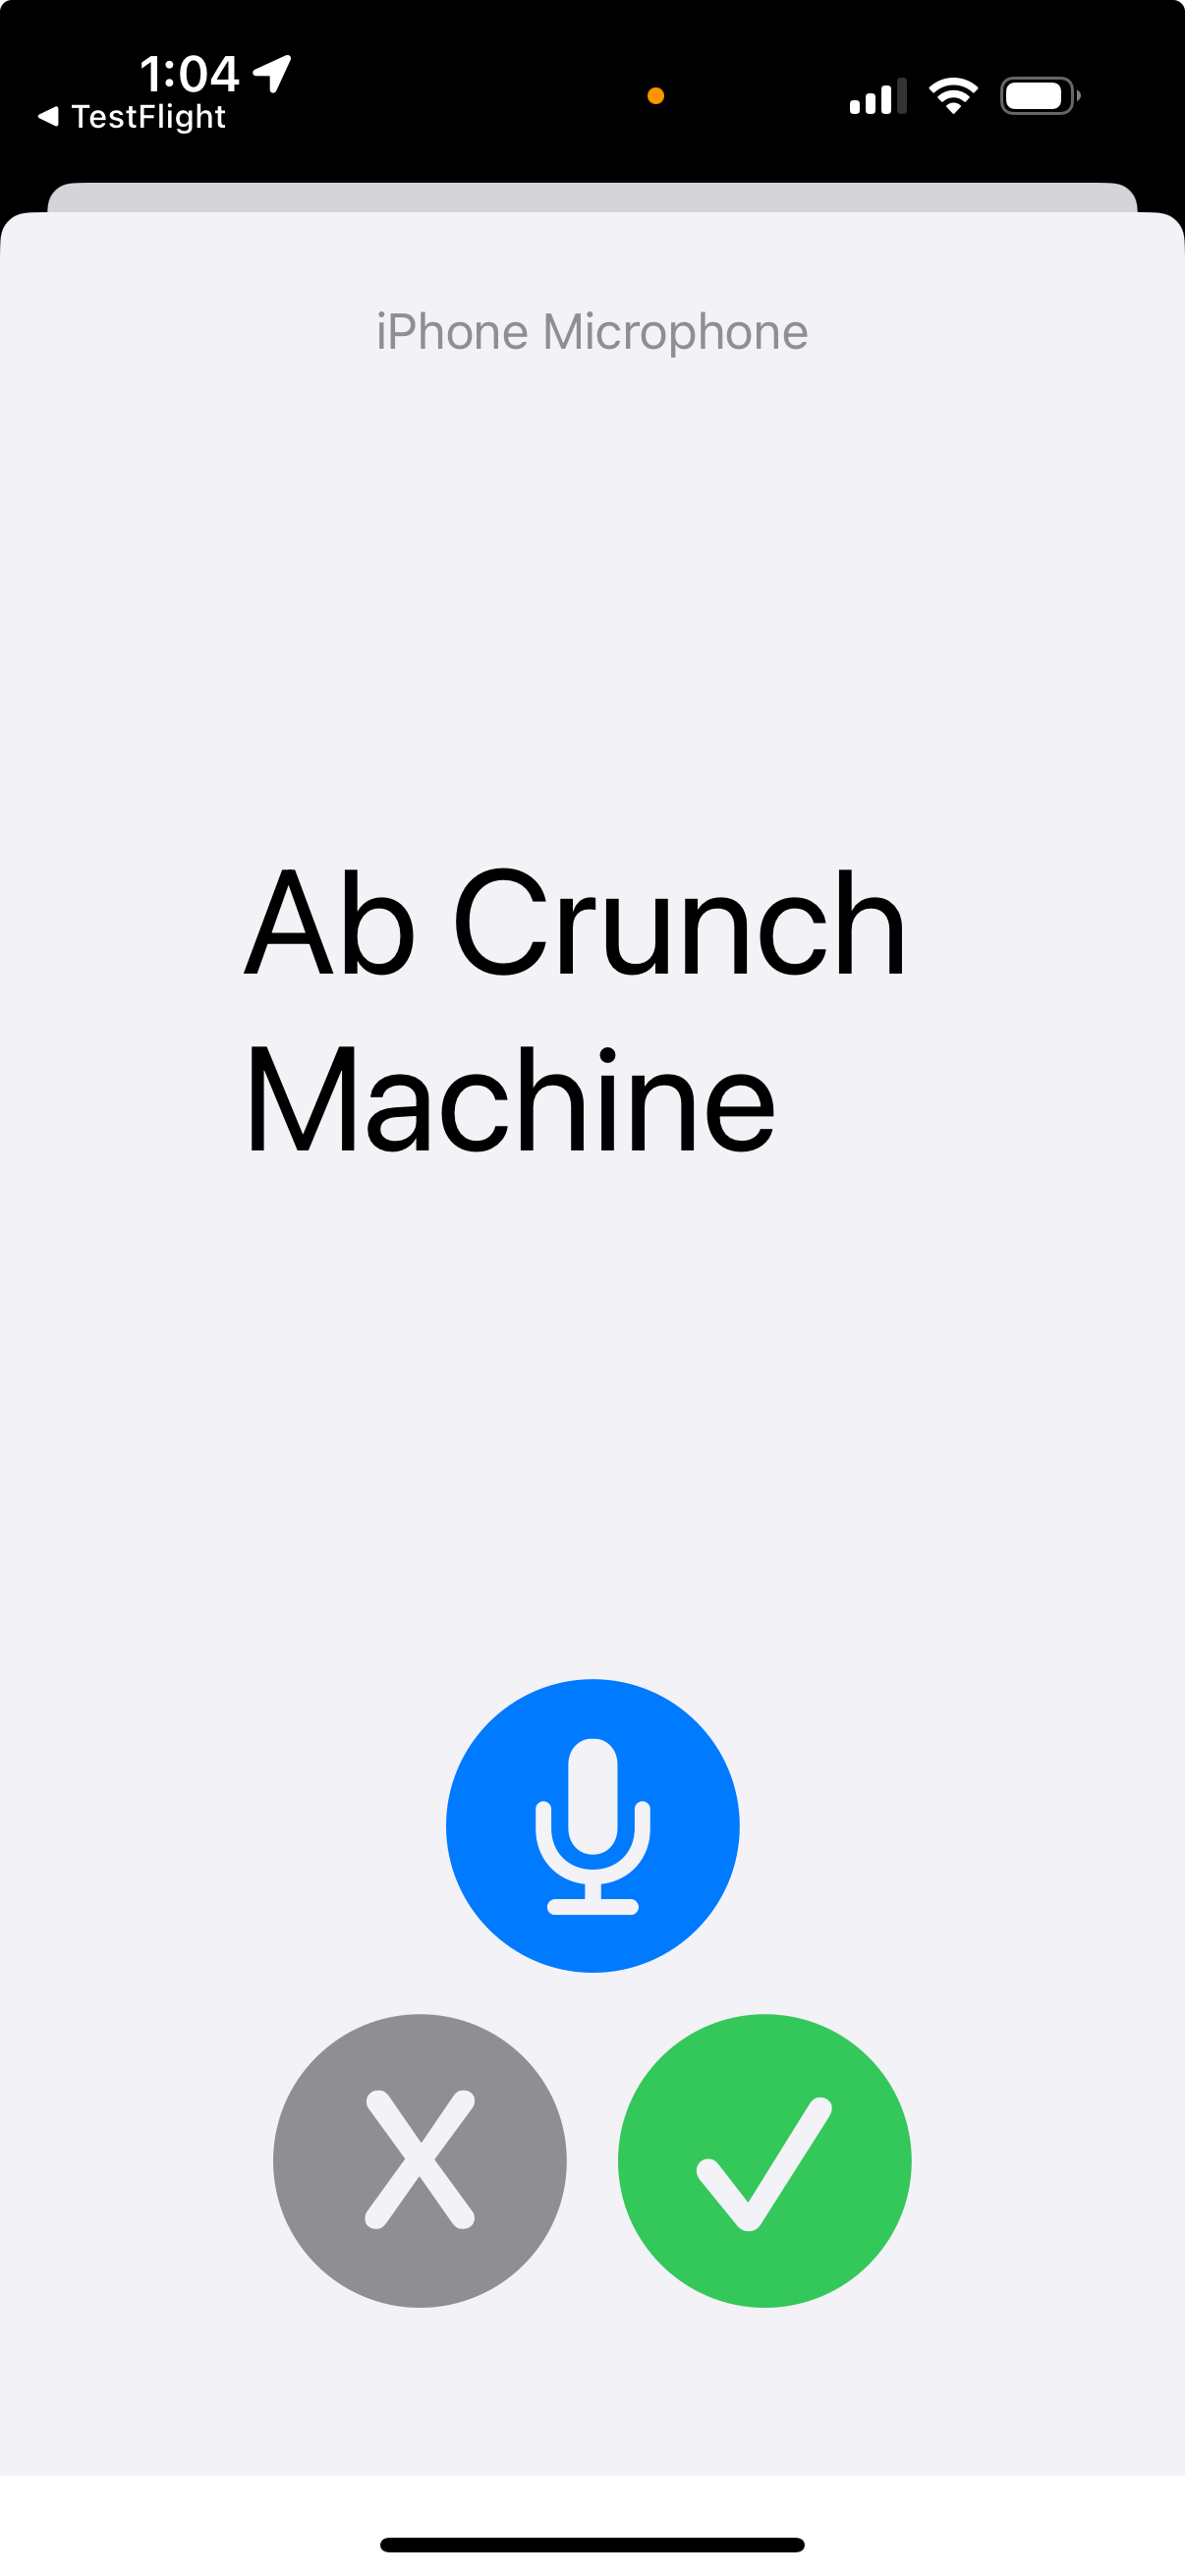
\includegraphics[height=8cm]{images/scasr.png}
\end{column}
\end{columns}
\end{frame}

\begin{frame}
\frametitle{Prototype case: Gym Working Logging App}
\begin{columns}
\begin{column}{0.5\textwidth}
The iOS app is a polished minimum-viable product that will be launched soon from the time of creating this presentation.
\end{column}
\begin{column}{0.5\textwidth}
    \centering
    
\includegraphics[height=3cm]{images/sc_icon.png}
\end{column}
\end{columns}
\end{frame}

\begin{frame}
\frametitle{Prototype case: Gym Working Logging App}
Research results below compares ``Custom" to SaaS APIs demonstrate the need for better contextualizing tools \\
\vspace{1cm}
\centering
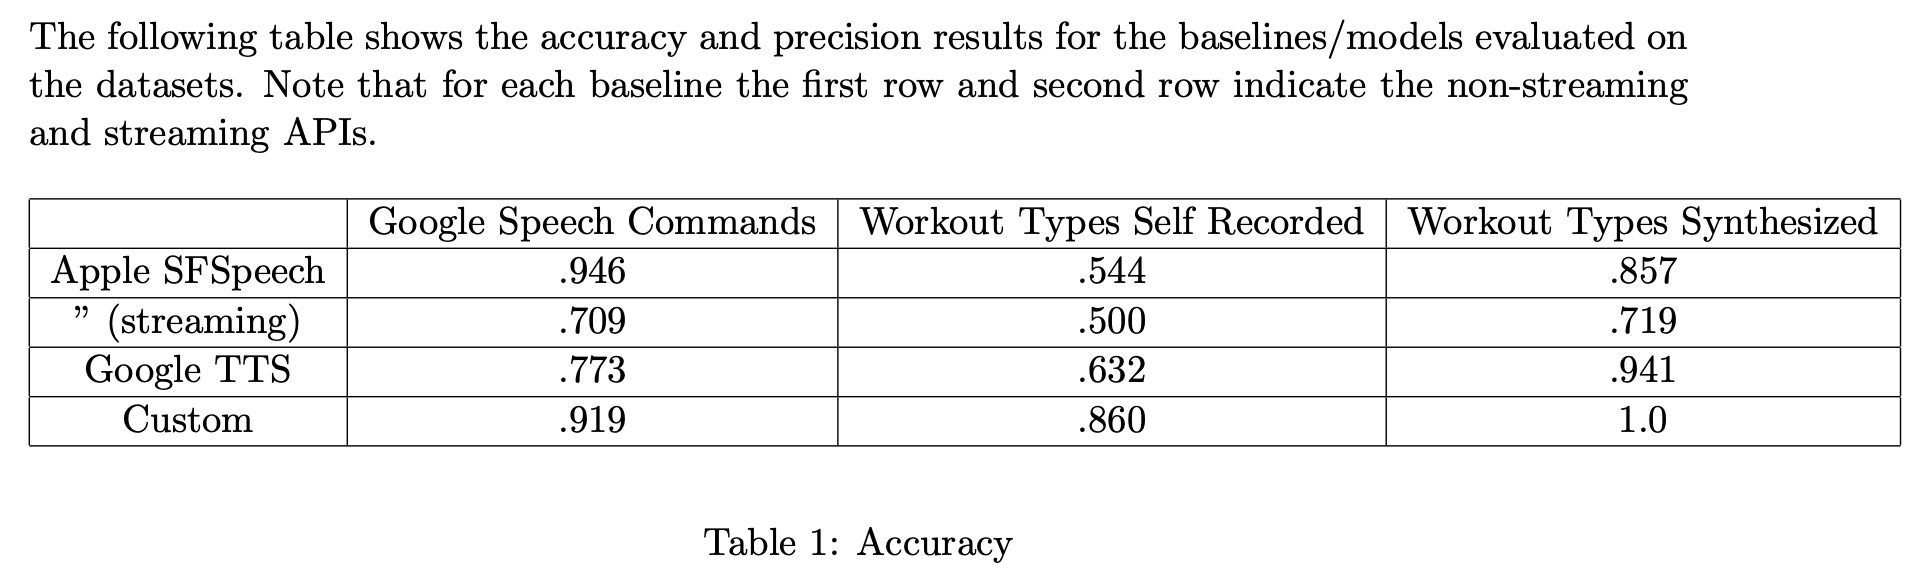
\includegraphics[height=3cm]{images/preliminary_results.png}
\end{frame}

\begin{frame}
\frametitle{Prototype case: Gym Working Logging App}
For a whitepaper that delves further in the technical aspects and justification, visit \\
\vspace{1cm}
\url{https://cs.brown.edu/people/ycheng79/csci1952qs23/Top_Project_3_Christopher\%20Hong_Low\%20Latency\%20Streaming\%20Speech\%20Selection.pdf}
\end{frame}

\begin{frame}
\frametitle{Other Potential Markets}
\begin{itemize}
    \item A Desktop app for personal trainers to quickly organize routines for their clients
    \item Voice control for people with upper-body physical impairments
    \item Field operators (in various industries) who need quick access to proprietary information
\end{itemize}
\end{frame}

\begin{frame}
\frametitle{A Disruptive, General Purpose Technology}
\begin{itemize}
    \item Context aware short-form speech recognition is potentially a \textit{disruptive} technology, in the sense used in \href{https://www.amazon.com/Innovators-Dilemma-Technologies-Management-Innovation/dp/1633691780}{The Innovator's Dilemma}
    \item Big Tech's strategy with voice assistants is to be useful to a wide swath of customers and gravitate them towards their own product ecosystem
    \item However, this leads voice assistants to be useful to nobody
    \item The right approach is to meet the needs of niche applications first
    \item In the end, the invested technology and capabilities can grow into mass-market general purpose technology of connecting voice to code 
\end{itemize}

\end{frame}

\end{document}
